\documentclass{article}

% content/resources/templates/preamble.tex
\usepackage[margin=0.6in]{geometry}
\author{Milav Dabgar}
\usepackage{amsmath,amssymb,amsthm}
\usepackage{booktabs}
\usepackage{multirow}
\usepackage{xcolor}
\usepackage{tcolorbox}
\tcbuselibrary{breakable,skins}
\usepackage[colorlinks=true,linkcolor=blue]{hyperref}
\usepackage{titlesec}
\usepackage{enumitem}
\usepackage{tikz}
\usepackage{pgfplots}
\usepackage{circuitikz}
\usepackage[version=4]{mhchem}
\usepackage{longtable}
\usepackage{array}
\usepackage{float}
\usepackage{caption}
\usepackage{listings}

\lstset{
  basicstyle=\small\ttfamily,
  breaklines=true,
  breakatwhitespace=false,
  postbreak=\mbox{\textcolor{red}{$\hookrightarrow$}\space},
  float=false,
  numbers=left,
  numberstyle=\tiny\color{gray},
  numbersep=10pt,
  xleftmargin=2em,
  keywordstyle=\color{blue},
  commentstyle=\color{green!60!black},
  stringstyle=\color{purple},
  backgroundcolor=\color{gray!5},
  showstringspaces=false,
  tabsize=2,
  captionpos=b,
  keepspaces=true,
  columns=flexible
}

\pgfplotsset{compat=1.18}
\usetikzlibrary{shapes,arrows,positioning,calc,patterns,decorations.pathmorphing,decorations.markings,arrows.meta}

% Color scheme
\definecolor{headcolor}{RGB}{0,102,204}
\definecolor{keycolor}{RGB}{220,20,60}
\definecolor{solutioncolor}{RGB}{34,139,34}
\definecolor{mnemoniccolor}{RGB}{148,0,211}
\definecolor{codecolor}{RGB}{0,0,100}

% Spacing
\setlength{\parskip}{3pt}
\setlist[itemize]{nosep}
\setlist[enumerate]{nosep}

% Title formatting
\titleformat{\section}{\Large\bfseries\color{headcolor}}{\thesection}{1em}{}
\titleformat{\subsection}{\large\bfseries\color{headcolor}}{\thesubsection}{1em}{}

% Pandoc tightlist compatibility
\providecommand{\tightlist}{%
  \setlength{\itemsep}{0pt}\setlength{\parskip}{0pt}}

% Pandoc longtable compatibility
\newcounter{none}
\def\thenone{}


% content/resources/templates/english-boxes.tex

% Custom environments
\newtcolorbox{solutionbox}{
 breakable,
 enhanced,
 colback=solutioncolor!5!white,
 colframe=solutioncolor!75!black,
 fonttitle=\bfseries,
 title=Solution
}

\newtcolorbox{solutionboxnobreak}{
 colback=solutioncolor!5!white,
 colframe=solutioncolor!75!black,
 fonttitle=\bfseries,
 title=Solution
}

\newtcolorbox{keyformula}{
 breakable,
 enhanced,
 colback=keycolor!5!white,
 colframe=keycolor!75!black,
 fonttitle=\bfseries,
 title=Key Formula
}

\newtcolorbox{mnemonicboxenv}{
 breakable,
 enhanced,
 colback=mnemoniccolor!5!white,
 colframe=mnemoniccolor!75!black,
 fonttitle=\bfseries,
 title=Mnemonic
}

\newcommand{\mnemonicbox}[1]{%
  \begin{mnemonicboxenv}
    #1
  \end{mnemonicboxenv}
}


% Custom commands for GTU solutions
% This file defines semantic commands for consistent formatting

% Question command with automatic formatting
\newcommand{\question}[2]{%
  \section*{Question #1}%
  \textbf{#2}%
}

% OR question variant
\newcommand{\questionor}[2]{%
  \section*{Question #1 OR}%
  \textbf{#2}%
}

% Proper table environment with caption
\newenvironment{answertable}[1]{%
  \begin{table}[htbp]
  \centering
  \caption{#1}
}{%
  \end{table}
}

% Proper figure environment for diagrams
\newenvironment{answerdiagram}[1]{%
  \begin{figure}[htbp]
  \centering
  \caption{#1}
}{%
  \end{figure}
}

% Semantic markup for key terms
\newcommand{\keyword}[1]{\textbf{#1}}
\newcommand{\code}[1]{\texttt{#1}}
\newcommand{\classname}[1]{\texttt{#1}}
\newcommand{\methodname}[1]{\texttt{#1}}

% Proper quotation marks
\newcommand{\mnemonic}[1]{``#1''}


\title{Microwave and Radar Communication (4351103) - Summer 2024 Solution}
\date{May 21, 2024}

\begin{document}
\maketitle

\questionmarks{1(a)}{3}{List different microwave bands with their frequency range.}

\begin{solutionbox}
\textbf{Microwave Frequency Bands:}

\begin{answertable}{Microwave Frequency Bands}
\begin{tabulary}{\linewidth}{|L|L|L|}
\hline
\textbf{Band} & \textbf{Frequency Range} & \textbf{Wavelength} \\ \hline
\keyword{L Band} & 1-2 GHz & 30-15 cm \\ \hline
\keyword{S Band} & 2-4 GHz & 15-7.5 cm \\ \hline
\keyword{C Band} & 4-8 GHz & 7.5-3.75 cm \\ \hline
\keyword{X Band} & 8-12 GHz & 3.75-2.5 cm \\ \hline
\keyword{Ku Band} & 12-18 GHz & 2.5-1.67 cm \\ \hline
\keyword{K Band} & 18-27 GHz & 1.67-1.11 cm \\ \hline
\keyword{Ka Band} & 27-40 GHz & 1.11-0.75 cm \\ \hline
\end{tabulary}
\end{answertable}
\end{solutionbox}

\begin{mnemonicbox}
\mnemonic{Large Ships Can eXamine Kindly Using Knowledge Always}
\end{mnemonicbox}

\questionmarks{1(b)}{4}{Draw the general equivalent circuit of the transmission line. Write the equation for characteristic impedance for a lossless line.}

\begin{solutionbox}
\textbf{Transmission Line Equivalent Circuit:}

\begin{answerdiagram}{Transmission Line Model}
\begin{center}
\begin{circuitikz}[american voltages]
    \draw (0,2) to[R, l=$R$, -*] (2,2) to[L, l=$L$, -*] (4,2) -- (5,2);
    \draw (4,2) to[C, l=$C$, *-*] (4,0);
    \draw (3,2) -- (3,1.5) to[R, l=$G$] (3,0.5) -- (3,0);
    \draw (0,0) to[short, -*] (5,0);
    
    \node at (2.5, -0.5) {$\Delta x$};
    \node [anchor=east] at (0,2) {Input};
    \node [anchor=west] at (5,2) {Output};
\end{circuitikz}
\end{center}
\end{answerdiagram}

\textbf{Circuit Elements:}
\begin{itemize}
    \item \keyword{R}: Series resistance per unit length
    \item \keyword{L}: Series inductance per unit length
    \item \keyword{C}: Shunt capacitance per unit length
    \item \keyword{G}: Shunt conductance per unit length
\end{itemize}

\textbf{For Lossless Line ($R=0, G=0$):}
\[ Z_0 = \sqrt{\frac{L}{C}} \]

\textbf{Key Points:}
\begin{itemize}
    \item \keyword{Lossless condition}: No power loss during transmission.
    \item \keyword{Impedance matching}: $Z_0$ determines reflection behavior.
\end{itemize}
\end{solutionbox}

\begin{mnemonicbox}
\mnemonic{Lossless Lines Love Constant Impedance}
\end{mnemonicbox}

\questionmarks{1(c)}{7}{Explain the impedance matching process using a single stub.}

\begin{solutionbox}
\textbf{Single Stub Matching Process:}

\begin{answerdiagram}{Single Stub Matching}
\begin{tikzpicture}[auto, node distance=2cm]
    \node [gtu block] (source) {Source};
    \node [gtu block, right=of source] (stub_point) {Junction Point};
    \node [gtu block, right=of stub_point] (load) {Load ($Z_L$)};
    \node [gtu block, below=of stub_point] (stub) {Short/Open Stub};

    \draw [gtu arrow] (source) -- node[above] {Main Line} (stub_point);
    \draw [gtu arrow] (stub_point) -- node[above] {Distance $d$} (load);
    \draw [gtu arrow] (stub) -- node[right] {Length $l$} (stub_point);
\end{tikzpicture}
\end{answerdiagram}

\textbf{Matching Steps:}
\begin{answertable}{Matching Procedure}
\begin{tabulary}{\linewidth}{|C|L|L|}
\hline
\textbf{Step} & \textbf{Process} & \textbf{Purpose} \\ \hline
1 & Calculate load admittance & Find $Y_L = 1/Z_L$ \\ \hline
2 & Move toward generator & Find point where $G = G_0$ \\ \hline
3 & Add stub susceptance & Cancel reactive part \\ \hline
4 & Achieve matching & $Y_{total} = Y_0$ \\ \hline
\end{tabulary}
\end{answertable}

\textbf{Design Equations:}
\begin{itemize}
    \item \keyword{Distance to stub}: $d = (\lambda/2\pi) \times \tan^{-1}(\sqrt{R_L/R_0})$
    \item \keyword{Stub length}: $l = (\lambda/2\pi) \times \tan^{-1}(B_{stub}/Y_0)$
\end{itemize}

\textbf{Applications:} Antenna matching, Amplifier input/output, Filter design.
\end{solutionbox}

\begin{mnemonicbox}
\mnemonic{Single Stubs Stop Standing Waves Successfully}
\end{mnemonicbox}

\orquestionmarks{1(c)}{7}{Compare rectangular and circular waveguides.}

\begin{solutionbox}
\textbf{Comparison:}

\begin{answertable}{Rectangular vs Circular Waveguide}
\begin{tabulary}{\linewidth}{|L|L|L|}
\hline
\textbf{Parameter} & \textbf{Rectangular Waveguide} & \textbf{Circular Waveguide} \\ \hline
\keyword{Shape} & Rectangular cross-section & Circular cross-section \\ \hline
\keyword{Dominant Mode} & $TE_{10}$ & $TE_{11}$ \\ \hline
\keyword{Cutoff Frequency} & $f_c = c/(2a)$ for $TE_{10}$ & $f_c = 1.841c/(2\pi a)$ for $TE_{11}$ \\ \hline
\keyword{Power Handling} & Lower & Higher \\ \hline
\keyword{Manufacturing} & Easy & Difficult \\ \hline
\keyword{Mode Separation} & Good & Poor \\ \hline
\keyword{Applications} & Radar, microwave ovens & Satellite communication \\ \hline
\end{tabulary}
\end{answertable}

\textbf{Key Advantages:}
\begin{itemize}
    \item \keyword{Rectangular}: Better mode control, easier fabrication.
    \item \keyword{Circular}: Higher power capacity, rotating polarization.
\end{itemize}
\end{solutionbox}

\begin{mnemonicbox}
\mnemonic{Rectangular is Regular, Circular Carries Current}
\end{mnemonicbox}

\questionmarks{2(a)}{3}{Define group velocity and phase velocity in relation to them.}

\begin{solutionbox}
\textbf{Velocity Definitions:}

\begin{answertable}{Velocity Types}
\begin{tabulary}{\linewidth}{|L|L|L|}
\hline
\textbf{Velocity Type} & \textbf{Formula} & \textbf{Physical Meaning} \\ \hline
\keyword{Phase Velocity} & $v_p = \omega/\beta = c/\sqrt{1-(f_c/f)^2}$ & Speed of constant phase \\ \hline
\keyword{Group Velocity} & $v_g = d\omega/d\beta = c\sqrt{1-(f_c/f)^2}$ & Speed of signal energy \\ \hline
\end{tabulary}
\end{answertable}

\textbf{Relationship:} $v_p \times v_g = c^2$

\textbf{Key Points:}
\begin{itemize}
    \item \keyword{Phase velocity}: Always $> c$ (speed of light).
    \item \keyword{Group velocity}: Always $< c$.
    \item \keyword{Signal travels}: At group velocity.
\end{itemize}
\end{solutionbox}

\begin{mnemonicbox}
\mnemonic{Phase is Fast, Group Carries Message}
\end{mnemonicbox}

\questionmarks{2(b)}{4}{Describe the principles and workings of the Directional coupler.}

\begin{solutionbox}
\textbf{Directional Coupler Principle:}

\begin{answerdiagram}{Directional Coupler}
\begin{tikzpicture}[auto, node distance=2cm]
    \node [gtu block, minimum width=3cm] (main) {Main Line};
    \node [gtu block, minimum width=3cm, below=1cm of main] (aux) {Auxiliary Line};
    
    \node [left=of main] (p1) {Port 1 (Input)};
    \node [right=of main] (p2) {Port 2 (Through)};
    \node [left=of aux] (p3) {Port 3 (Coupled)};
    \node [right=of aux] (p4) {Port 4 (Isolated)};
    
    \draw [gtu arrow] (p1) -- (main);
    \draw [gtu arrow] (main) -- (p2);
    \draw [gtu dotted arrow] (main) -- node[midway, right] {Coupling} (aux);
    \draw [gtu arrow] (aux) -- (p3);
    \draw [gtu arrow] (aux) -- (p4);
\end{tikzpicture}
\end{answerdiagram}

\textbf{Key Parameters:}
\begin{itemize}
    \item \keyword{Coupling Factor}: $C = 10 \log(P_1/P_3)$ dB
    \item \keyword{Directivity}: $D = 10 \log(P_3/P_4)$ dB
    \item \keyword{Insertion Loss}: $IL = 10 \log(P_1/P_2)$ dB
\end{itemize}
\end{solutionbox}

\begin{mnemonicbox}
\mnemonic{Directional Couplers Divide Power Precisely}
\end{mnemonicbox}

\questionmarks{2(c)}{7}{Explain Magic TEE with construction, operation and application.}

\begin{solutionbox}
\textbf{Magic TEE Construction:}

\begin{answerdiagram}{Magic TEE Structure}
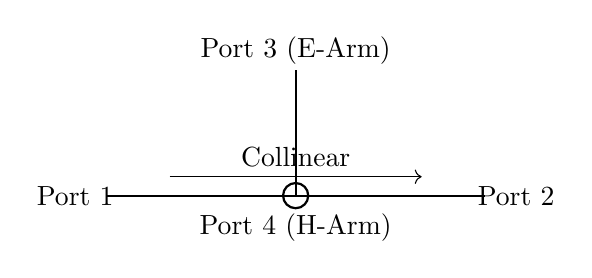
\begin{tikzpicture}[scale=0.8]
    % Simple TEE representation
    \draw[thick] (-3,0) -- (3,0); % Main arm
    \draw[thick] (0,0) -- (0,2);  % E-arm
    \draw[thick] (0,0) circle (0.2); % H-arm sticking out
    
    \node at (-3.5,0) {Port 1};
    \node at (3.5,0) {Port 2};
    \node at (0,2.3) {Port 3 (E-Arm)};
    \node at (0,-0.5) {Port 4 (H-Arm)};
    
    \draw[->] (-2,0.3) -- node[above] {Collinear} (2,0.3);
\end{tikzpicture}
\end{answerdiagram}

\textbf{Operating Principles:}
\begin{answertable}{Port Functions}
\begin{tabulary}{\linewidth}{|L|L|L|}
\hline
\textbf{Port} & \textbf{Function} & \textbf{Field Pattern} \\ \hline
\keyword{Port 1 \& 2} & Collinear ports & Symmetric \\ \hline
\keyword{Port 3 (E-Arm)} & E-plane port & Difference port ($P_1 - P_2$) \\ \hline
\keyword{Port 4 (H-Arm)} & H-plane port & Sum port ($P_1 + P_2$) \\ \hline
\end{tabulary}
\end{answertable}

\textbf{Properties:}
\begin{itemize}
    \item \keyword{Isolation}: Port 3 isolated from Port 4.
    \item \keyword{Power division}: Equal split when matched.
\end{itemize}

\textbf{Applications:} Mixers, Power combiners, Impedance bridges.
\end{solutionbox}

\begin{mnemonicbox}
\mnemonic{Magic TEE Creates Perfect Isolation}
\end{mnemonicbox}

\orquestionmarks{2(a)}{3}{Draw TE$_{10}$, TE$_{20}$ modes for rectangular waveguide.}

\begin{solutionbox}
\textbf{TE$_{10}$ Mode (Dominant):}

\begin{answerdiagram}{TE Modes}
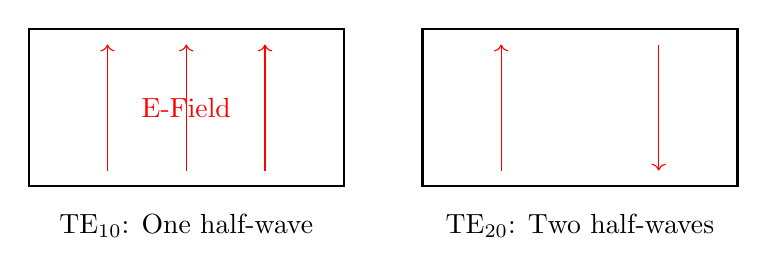
\begin{tikzpicture}
    % TE10
    \draw[thick] (0,0) rectangle (4,2);
    \node at (2, -0.5) {TE$_{10}$: One half-wave};
    \foreach \x in {1, 2, 3} {
        \draw[->, red] (\x, 0.2) -- (\x, 1.8);
    }
    \node[red] at (2,1) {E-Field};

    % TE20
    \begin{scope}[xshift=5cm]
    \draw[thick] (0,0) rectangle (4,2);
    \node at (2, -0.5) {TE$_{20}$: Two half-waves};
    \draw[->, red] (1, 0.2) -- (1, 1.8);
    \draw[->, red] (3, 1.8) -- (3, 0.2);
    \end{scope}
\end{tikzpicture}
\end{answerdiagram}

\textbf{Characteristics:}
\begin{itemize}
    \item \keyword{TE10}: Single half-wave variation across broad dimension $a$.
    \item \keyword{TE20}: Two half-wave variations across $a$.
\end{itemize}
\end{solutionbox}

\begin{mnemonicbox}
\mnemonic{TE modes have Electric Transverse}
\end{mnemonicbox}

\orquestionmarks{2(b)}{4}{Describe the Hybrid Ring with a necessary sketch.}

\begin{solutionbox}
\textbf{Hybrid Ring Structure:}

\begin{answerdiagram}{Rat-Race Coupler}
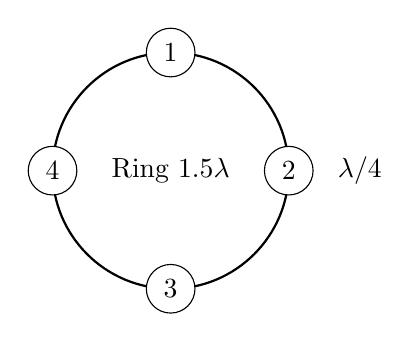
\begin{tikzpicture}
    \draw[thick] (0,0) circle (1.5);
    \node at (0,0) {Ring $1.5\lambda$};
    
    \node[draw, circle, fill=white] (p1) at (90:1.5) {1};
    \node[draw, circle, fill=white] (p2) at (0:1.5) {2};
    \node[draw, circle, fill=white] (p3) at (-90:1.5) {3};
    \node[draw, circle, fill=white] (p4) at (180:1.5) {4};
    
    \node[right] at (2,0) {$\lambda/4$};
   
\end{tikzpicture}
\end{answerdiagram}

\textbf{Operating Principle:}
\begin{itemize}
    \item \keyword{Circumference}: $3\lambda/2$ ($1.5\lambda$).
    \item \keyword{Port Spacing}: Ports are spaced $\lambda/4$ apart, except one gap is $3\lambda/4$.
    \item \keyword{Isolation}: Specific ports are isolated due to phase cancellation.
\end{itemize}
\end{solutionbox}

\begin{mnemonicbox}
\mnemonic{Hybrid Rings Handle Half-wavelengths}
\end{mnemonicbox}

\orquestionmarks{2(c)}{7}{Explain the Isolator with principles, construction and operation.}

\begin{solutionbox}
\textbf{Isolator Principle:}

\begin{answerdiagram}{Isolator}
\begin{tikzpicture}[auto, node distance=2cm]
    \node [gtu state] (input) {Input};
    \node [gtu block, right=of input, fill=gray!20] (ferrite) {Ferrite\\Material};
    \node [gtu state, right=of ferrite] (output) {Output};
    
    \draw [gtu arrow] (input) -- (ferrite);
    \draw [gtu arrow] (ferrite) -- (output);
    
    \draw [->, red, dashed] (output) to[bend right] node[above] {Blocked} (ferrite);
    
    \node [above=of ferrite] (magnet) {Permanent Magnet ($B$)};
    \draw [->] (magnet) -- (ferrite);
\end{tikzpicture}
\end{answerdiagram}

\textbf{Key Elements:}
\begin{itemize}
    \item \keyword{Ferrite}: Non-reciprocal material (e.g., Yttrium Iron Garnet).
    \item \keyword{Magnet}: Provides bias magnetic field.
    \item \keyword{Card}: Absorptive resistive card to kill reverse power.
\end{itemize}

\textbf{Operation:} Based on \keyword{Faraday Rotation}. Forward wave passes with little loss. Reverse wave is rotated such that it is absorbed by the resistive card (Attenuated).
\end{solutionbox}

\begin{mnemonicbox}
\mnemonic{Isolators Ignore Reverse Reflections}
\end{mnemonicbox}

\questionmarks{3(a)}{3}{Draw a Traveling wave tube amplifier.}

\begin{solutionbox}
\textbf{TWT Amplifier:}

\begin{answerdiagram}{TWT Structure}
\begin{tikzpicture}[auto, node distance=1.5cm]
    \node [gtu start] (gun) {Electron\\Gun};
    \node [gtu block, right=of gun, shape=cylinder, shape border rotate=0, aspect=0.2, minimum width=4cm] (helix) {Helix Slow-Wave Structure};
    \node [gtu stop, right=of helix] (collector) {Collector};
    
    \draw [gtu arrow] (gun) -- (helix);
    \draw [gtu arrow] (helix) -- (collector);
    
    \node [above=0.5cm of helix] (in) {RF Input};
    \node [above=0.5cm of collector] (out) {RF Output};
    
    \draw [->] (in) -- (helix.north west);
    \draw [<-] (out) -- (helix.north east);
    
    \node [below=0.5cm of helix] {Attenuator};
\end{tikzpicture}
\end{answerdiagram}
\end{solutionbox}

\begin{mnemonicbox}
\mnemonic{TWT Transfers Wave Through Helix}
\end{mnemonicbox}

\questionmarks{3(b)}{4}{Describes various types of hazards due to microwave radiation.}

\begin{solutionbox}
\textbf{Microwave Hazards:}

\begin{answertable}{Radiation Hazards}
\begin{tabulary}{\linewidth}{|L|L|L|}
\hline
\textbf{Hazard Type} & \textbf{Effects} & \textbf{Limit} \\ \hline
\keyword{HERP} (Personnel) & Tissue heating, cataracts, burns & 10 mW/cm$^2$ \\ \hline
\keyword{HERO} (Ordnance) & Accidental detonation of explosives & Variable \\ \hline
\keyword{HERF} (Fuel) & Fuel ignition/sparks & 5 mW/cm$^2$ \\ \hline
\end{tabulary}
\end{answertable}

\textbf{Biological Effects:}
\begin{itemize}
    \item \keyword{Thermal}: Heating of water-rich tissues (eyes, brain, stomach).
    \item \keyword{Non-thermal}: Potential DNA/cellular effects (debated).
\end{itemize}

\textbf{Protection:} Shielding, Distance ($1/r^2$ law), Time limits.
\end{solutionbox}

\begin{mnemonicbox}
\mnemonic{Heat Energy Requires Proper Protection}
\end{mnemonicbox}

\questionmarks{3(c)}{7}{Explain two cavity klystrons construction and operation with an Applegate diagram.}

\begin{solutionbox}
\textbf{Two-Cavity Klystron Construction:}

\begin{answerdiagram}{Klystron Block Diagram}
\begin{tikzpicture}[auto, node distance=1.5cm]
    \node [gtu start] (cathode) {Cathode};
    \node [gtu block, right=of cathode] (buncher) {Buncher\\Cavity};
    \node [gtu block, right=of buncher, minimum width=2cm] (drift) {Drift Space};
    \node [gtu block, right=of drift] (catcher) {Catcher\\Cavity};
    \node [gtu stop, right=of catcher] (collector) {Collector};
    
    \draw [gtu arrow] (cathode) -- (buncher);
    \draw [gtu arrow] (buncher) -- (drift);
    \draw [gtu arrow] (drift) -- (catcher);
    \draw [gtu arrow] (catcher) -- (collector);
    
    \node [above=of buncher] {RF Input};
    \node [above=of catcher] {RF Output};
\end{tikzpicture}
\end{answerdiagram}

\textbf{Applegate Diagram (Bunching Process):}

\begin{answerdiagram}{Applegate Diagram}
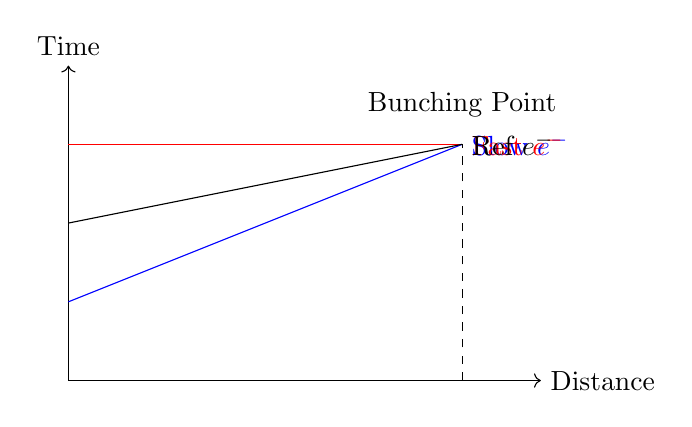
\begin{tikzpicture}
    \draw[->] (0,0) -- (6,0) node[right] {Distance};
    \draw[->] (0,0) -- (0,4) node[above] {Time};
    
    % Electron paths
    \draw[blue] (0,1) -- (5,3) node[right] {Slow $e^-$};
    \draw[red] (0,3) -- (5,3) node[right] {Fast $e^-$};
    \draw[black] (0,2) -- (5,3) node[right] {Ref $e^-$};
    
    \node at (5,3.5) {Bunching Point};
    \draw[dashed] (5,0) -- (5,3);
\end{tikzpicture}
\end{answerdiagram}

\textbf{Operation Principles:}
\begin{itemize}
    \item \keyword{Velocity Modulation}: RF input accelerates/decelerates electrons in Buncher cavity.
    \item \keyword{Drift Space}: Fast electrons catch up to slow ones, forming electron bunches.
    \item \keyword{Energy Extraction}: Bunches induce strong oscillations in Catcher cavity.
\end{itemize}
\end{solutionbox}

\begin{mnemonicbox}
\mnemonic{Klystrons Create Bunches Through Velocity Variation}
\end{mnemonicbox}

\orquestionmarks{3(a)}{3}{Draw the block diagram of the attenuation measurement method for microwave frequency.}

\begin{solutionbox}
\textbf{Attenuation Measurement:}

\begin{answerdiagram}{Attenuation Setup}
\begin{tikzpicture}[auto, node distance=1.5cm]
    \node [gtu input] (gen) {Signal\\Gen};
    \node [gtu block, right=of gen] (iso) {Isolator};
    \node [gtu block, right=of iso] (dut) {Device Under\\Test (DUT)};
    \node [gtu block, right=of dut] (det) {Detector};
    \node [gtu output, right=of det] (meter) {Power\\Meter};
    
    \draw [gtu arrow] (gen) -- (iso);
    \draw [gtu arrow] (iso) -- (dut);
    \draw [gtu arrow] (dut) -- (det);
    \draw [gtu arrow] (det) -- (meter);
\end{tikzpicture}
\end{answerdiagram}

\textbf{Method:} Measure power $P_1$ without DUT, measure power $P_2$ with DUT. Attenuation (dB) $= 10 \log(P_1/P_2)$.
\end{solutionbox}

\begin{mnemonicbox}
\mnemonic{Attenuation Appears After Accurate Assessment}
\end{mnemonicbox}

\orquestionmarks{3(b)}{4}{Describe the limitation of vacuum tubes at microwave range.}

\begin{solutionbox}
\textbf{Limitations of Conventional Tubes:}

\begin{answertable}{Vacuum Tube Limitations}
\begin{tabulary}{\linewidth}{|L|L|L|}
\hline
\textbf{Limitation} & \textbf{Cause} & \textbf{Effect} \\ \hline
\keyword{Transit Time} & Finite electron velocity & Phase shift, reduced gain \\ \hline
\keyword{Lead Inductance} & Wiring inductance ($j\omega L$) & Impedance mismatch \\ \hline
\keyword{Inter-electrode C} & $C_{gp}, C_{gk}$ parasitics & Shunts signal, feedback \\ \hline
\keyword{Skin Effect} & Surface conduction & High resistance, loss \\ \hline
\end{tabulary}
\end{answertable}

\textbf{Consequences:} At $f > 1$ GHz, conventional tubes become oscillators or stop working entirely due to these parasitics.
\end{solutionbox}

\begin{mnemonicbox}
\mnemonic{Vacuum Tubes Fail Fast at High Frequencies}
\end{mnemonicbox}

\orquestionmarks{3(c)}{7}{Explain the Principle, construction, effect of the electric and magnetic field and operation of the magnetron in detail.}

\begin{solutionbox}
\textbf{Magnetron Construction:}

\begin{answerdiagram}{Magnetron Cross Section}
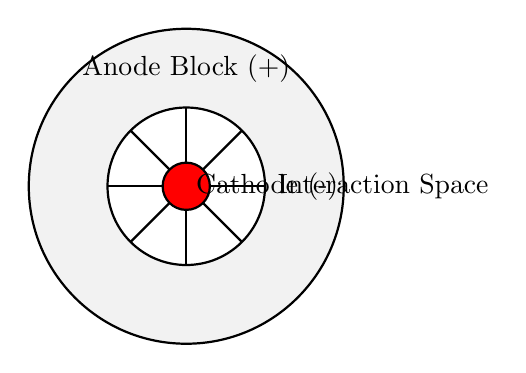
\begin{tikzpicture}
    % Anode block
    \draw[thick, fill=gray!10] (0,0) circle (2);
    \draw[thick, fill=white] (0,0) circle (1);
    
    % Vanes
    \foreach \angle in {0, 45, ..., 315} {
        \draw[thick] (0,0) -- (\angle:1);
    }
    
    % Cathode
    \draw[thick, fill=red] (0,0) circle (0.3);
    \node at (0,0) [right] { Cathode (-)};
    
    \node at (0, 1.5) {Anode Block (+)};
    \node at (2.5, 0) {Interaction Space};
\end{tikzpicture}
\end{answerdiagram}

\textbf{Principle of Operation:}
\begin{itemize}
    \item \keyword{Crossed Fields}: DC Electric field (Radial) and DC Magnetic field (Axial) are perpendicular.
    \item \keyword{Electron Motion}: Electrons emitted from cathode travel in cycloidal paths due to Lorentz force.
    \item \keyword{Interaction}: Electrons transfer potential energy to the RF field in cavities while spiraling outward.
\end{itemize}

\textbf{Hull Cutoff:}
\begin{itemize}
    \item If $B < B_c$: Electrons hit anode directly (High current).
    \item If $B > B_c$: Electrons miss anode and return to cathode (Cutoff).
    \item Oscillation occurs near the cutoff region.
\end{itemize}
\end{solutionbox}

\begin{mnemonicbox}
\mnemonic{Magnetrons Make Microwaves Through Magnetic Motion}
\end{mnemonicbox}

\questionmarks{4(a)}{3}{Explain the working principle of a varactor diode using a graph.}

\begin{solutionbox}
\textbf{Varactor Diode Characteristics:}

\begin{answerdiagram}{Varactor C-V Curve}
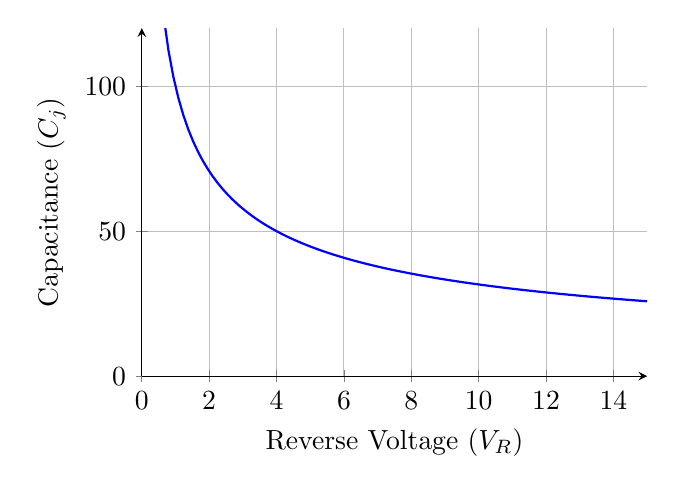
\begin{tikzpicture}
    \begin{axis}[
        axis lines = left,
        xlabel = {Reverse Voltage ($V_R$)},
        ylabel = {Capacitance ($C_j$)},
        ymin=0, ymax=120,
        xmin=0, xmax=15,
        grid=major,
        width=8cm,
        height=6cm
    ]
    \addplot [
        domain=0.5:15, 
        samples=100, 
        color=blue, 
        thick,
    ] {100/sqrt(x)};
    \end{axis}
\end{tikzpicture}
\end{answerdiagram}

\textbf{Working Principle:}
\begin{itemize}
    \item \keyword{Reverse Bias}: Operated in reverse bias mode.
    \item \keyword{Variable Capacitor}: Depletion layer width increases with reverse voltage.
    \item \keyword{Relation}: $C_j \propto 1/\sqrt{V_R + V_\phi}$. Higher voltage $\rightarrow$ Lower capacitance.
\end{itemize}

\textbf{Applications:} VCOs, Parametric Amplifiers, Frequency Multipliers.
\end{solutionbox}

\begin{mnemonicbox}
\mnemonic{Varactors Vary Capacitance Via Voltage}
\end{mnemonicbox}

\questionmarks{4(b)}{4}{Explain the Gunn Effect and negative resistance for Gunn diode.}

\begin{solutionbox}
\textbf{Gunn Effect (Transferred Electron Effect):}

\begin{answerdiagram}{Gunn Diode I-V Characteristic}
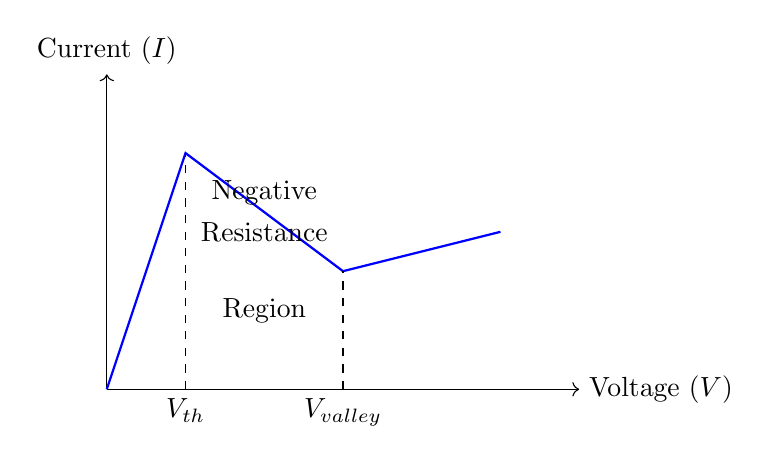
\begin{tikzpicture}
    \draw[->] (0,0) -- (6,0) node[right] {Voltage ($V$)};
    \draw[->] (0,0) -- (0,4) node[above] {Current ($I$)};
    
    \draw[thick, blue] (0,0) -- (1,3) -- (3,1.5) -- (5,2);
    
    \draw[dashed] (1,0) node[below] {$V_{th}$} -- (1,3);
    \draw[dashed] (3,0) node[below] {$V_{valley}$} -- (3,1.5);
    
    \node at (2, 2.5) {Negative};
    \node at (2, 2) {Resistance};
    \node at (2, 1) {Region};
\end{tikzpicture}
\end{answerdiagram}

\textbf{Mechanism:}
\begin{itemize}
    \item \keyword{Two Valleys}: Conductance band has lower valley (high mobility) and upper valley (low mobility).
    \item \keyword{Threshold}: Above $V_{th}$, electrons transfer to upper slow valley.
    \item \keyword{Negative Resistance}: Current decreases as voltage increases ($dI/dV < 0$), causing oscillations.
\end{itemize}
\end{solutionbox}

\begin{mnemonicbox}
\mnemonic{Gunn diodes Generate oscillations through Negative resistance}
\end{mnemonicbox}

\questionmarks{4(c)}{7}{Explain frequency measurement method for microwave frequency.}

\begin{solutionbox}
\textbf{Frequency Measurement Methods:}

\begin{answerdiagram}{Direct Frequency Counter}
\begin{tikzpicture}[auto, node distance=1.5cm]
    \node [gtu input] (sig) {Unknown\\Signal};
    \node [gtu block, right=of sig] (counter) {Microwave\\Frequency Counter};
    \node [gtu output, right=of counter] (disp) {Digital\\Display};
    \node [gtu block, below=of counter] (ref) {Crystal\\Reference};
    
    \draw [gtu arrow] (sig) -- (counter);
    \draw [gtu arrow] (counter) -- (disp);
    \draw [gtu arrow] (ref) -- (counter);
\end{tikzpicture}
\end{answerdiagram}

\textbf{Cavity Wavemeter (Indirect Method):}

\begin{answerdiagram}{Cavity Wavemeter}
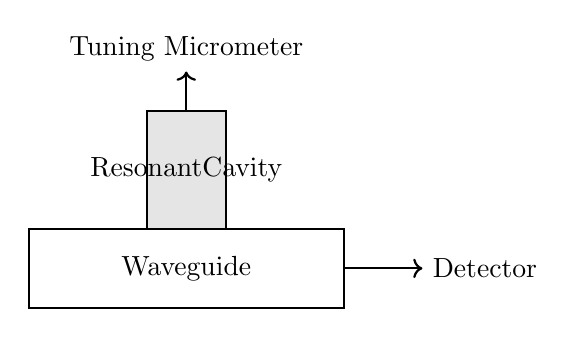
\begin{tikzpicture}
    \draw[thick] (0,0) rectangle (4,1);
    \node at (2,0.5) {Waveguide};
    
    \draw[thick, fill=gray!20] (1.5,1) rectangle (2.5,2.5);
    \node at (2,1.75) {Resonant\\Cavity};
    
    \draw[thick, ->] (2,2.5) -- (2,3) node[above] {Tuning Micrometer};
    
    \draw[thick, ->] (4,0.5) -- (5,0.5) node[right] {Detector};
\end{tikzpicture}
\end{answerdiagram}

\textbf{Procedure:}
\begin{enumerate}
    \item Couple wavemeter to transmission line.
    \item Tune the cavity plunger until resonance is observed (dip in power meter).
    \item Read frequency from the calibrated micrometer scale.
\end{enumerate}

\textbf{Heterodyne Method:} Mix unknown signal with local oscillator to generate beat frequency. $f_{unknown} = f_{LO} \pm f_{beat}$.
\end{solutionbox}

\begin{mnemonicbox}
\mnemonic{Frequency Found through Careful Cavity Calibration}
\end{mnemonicbox}

\orquestionmarks{4(a)}{3}{Explain the working of a PIN diode as a switch.}

\begin{solutionbox}
\textbf{PIN Diode Structure:}

\begin{answerdiagram}{PIN Diode}
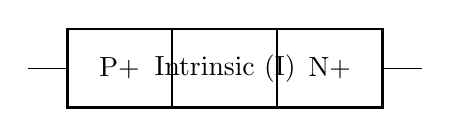
\begin{tikzpicture}
    \draw[thick] (0,0) rectangle (4,1);
    \draw[thick] (1.33,0) -- (1.33,1);
    \draw[thick] (2.66,0) -- (2.66,1);
    
    \node at (0.66, 0.5) {P+};
    \node at (2, 0.5) {Intrinsic (I)};
    \node at (3.33, 0.5) {N+};
    
    \draw (0,0.5) -- (-0.5,0.5);
    \draw (4,0.5) -- (4.5,0.5);
\end{tikzpicture}
\end{answerdiagram}

\textbf{Switching Action:}
\begin{answertable}{PIN Switch States}
\begin{tabulary}{\linewidth}{|L|L|L|}
\hline
\textbf{Bias} & \textbf{Intrinsic Region} & \textbf{State} \\ \hline
\keyword{Forward Bias} & Flooded with carriers (Low $R$) & \keyword{ON} (Pass signal) \\ \hline
\keyword{Reverse Bias} & Depleted (High $R$, Low $C$) & \keyword{OFF} (Block signal) \\ \hline
\end{tabulary}
\end{answertable}

\textbf{Advantages:} High power handling, Fast switching (ns), Wide bandwidth.
\end{solutionbox}

\begin{mnemonicbox}
\mnemonic{PIN diodes Perform Perfect switching}
\end{mnemonicbox}

\orquestionmarks{4(b)}{4}{Explain stripeline and Microstrip circuits.}

\begin{solutionbox}
\textbf{Comparison of Planar Transmission Lines:}

\begin{answerdiagram}{Stripline vs Microstrip}
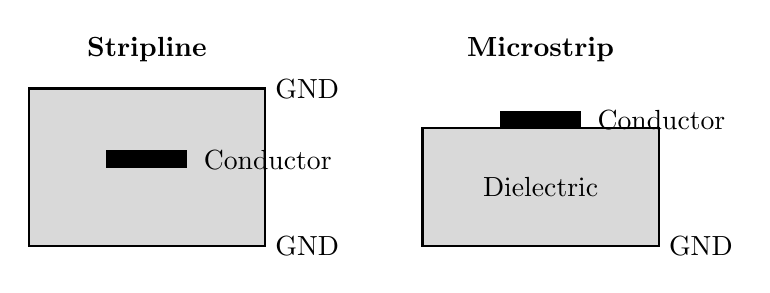
\begin{tikzpicture}
    % Stripline
    \begin{scope}
        \node at (1.5, 2.5) {\textbf{Stripline}};
        \draw[thick, fill=gray!30] (0,0) rectangle (3,2);
        \draw[thick] (0,0) -- (3,0) node[right] {GND};
        \draw[thick] (0,2) -- (3,2) node[right] {GND};
        \draw[thick, fill=black] (1,1) rectangle (2,1.2);
        \node at (1.5,1.1) [right=0.6cm] {Conductor};
    \end{scope}
    
    % Microstrip
    \begin{scope}[xshift=5cm]
        \node at (1.5, 2.5) {\textbf{Microstrip}};
        \draw[thick, fill=gray!30] (0,0) rectangle (3,1.5);
        \draw[thick] (0,0) -- (3,0) node[right] {GND};
        \draw[thick, fill=black] (1,1.5) rectangle (2,1.7);
        \node at (1.5,1.6) [right=0.6cm] {Conductor};
        \node at (1.5, 0.75) {Dielectric};
    \end{scope}
\end{tikzpicture}
\end{answerdiagram}

\begin{answertable}{Performance Comparison}
\begin{tabulary}{\linewidth}{|L|L|L|}
\hline
\textbf{Parameter} & \textbf{Stripline} & \textbf{Microstrip} \\ \hline
\keyword{Structure} & Conductor valid between 2 GNDs & Conductor on top of GND \\ \hline
\keyword{Radiation} & None (Shielded) & Radiates (Open top) \\ \hline
\keyword{Mode} & Pure TEM & Quasi-TEM \\ \hline
\keyword{Cost} & Higher (Complex PCB) & Lower (Simple PCB) \\ \hline
\end{tabulary}
\end{answertable}
\end{solutionbox}

\begin{mnemonicbox}
\mnemonic{Striplines are Sandwiched, Microstrips are Mounted}
\end{mnemonicbox}

\orquestionmarks{4(c)}{7}{Explain the principles and process of amplification for a Parametric amplifier.}

\begin{solutionbox}
\textbf{Parametric Amplifier Principle:}

\begin{answerdiagram}{Parametric Amplifier Block}
\begin{tikzpicture}[auto, node distance=2cm]
    \node [gtu decision] (nonlin) {Nonlinear\\Reactance\\(Varactor)};
    \node [gtu input, left=of nonlin] (sig) {Signal ($f_s$)};
    \node [gtu input, below=of nonlin] (pump) {Pump ($f_p$)};
    \node [gtu block, right=of nonlin] (idler) {Idler Circuit ($f_i$)};
    \node [gtu output, above=of nonlin] (out) {Output ($f_s$)};
    
    \draw [gtu arrow] (sig) -- (nonlin);
    \draw [gtu arrow] (pump) -- (nonlin);
    \draw [gtu arrow] (nonlin) -- (idler);
    \draw [gtu arrow] (nonlin) -- (out);
\end{tikzpicture}
\end{answerdiagram}

\textbf{Process:}
\begin{itemize}
    \item Uses a nonlinear reactance (Varactor diode) instead of resistance (low noise).
    \item \keyword{Pump Energy}: A high frequency pump ($f_p$) supplies energy to the system.
    \item \keyword{Mixing}: Interaction creates idler frequency $f_i = f_p - f_s$.
    \item \keyword{Amplification}: Energy is transferred from the Pump to the Signal frequency via the nonlinear capacitance.
\end{itemize}

\textbf{Advantages:} Extremely low noise figure (used in satellite/radio astronomy).
\end{solutionbox}

\begin{mnemonicbox}
\mnemonic{Parametric amplifiers Pump Power into signal Perfectly}
\end{mnemonicbox}

\questionmarks{5(a)}{3}{Compare RADAR and SONAR.}

\begin{solutionbox}
\textbf{Comparison:}

\begin{answertable}{RADAR vs SONAR}
\begin{tabulary}{\linewidth}{|L|L|L|}
\hline
\textbf{Parameter} & \textbf{RADAR} & \textbf{SONAR} \\ \hline
\keyword{Wave Type} & Electromagnetic (Radio) & Acoustic (Sound) \\ \hline
\keyword{Medium} & Air / Vacuum & Water \\ \hline
\keyword{Speed} & $3 \times 10^8$ m/s & ~1500 m/s \\ \hline
\keyword{Range} & Long (1000s km) & Short (< 100 km) \\ \hline
\keyword{Application} & Aviation, Weather & Submarine, Fishing \\ \hline
\end{tabulary}
\end{answertable}

\textbf{Principle:} Both use \keyword{Echo Ranging} ($R = vt/2$).
\end{solutionbox}

\begin{mnemonicbox}
\mnemonic{RADAR sees Radio waves, SONAR hears Sound waves}
\end{mnemonicbox}

\questionmarks{5(b)}{4}{Write the name of RADAR display method and explain anyone.}

\begin{solutionbox}
\textbf{RADAR Displays:} A-Scope, B-Scope, C-Scope, PPI (Plan Position Indicator), RHI.

\textbf{Plan Position Indicator (PPI):}

\begin{answerdiagram}{PPI Display}
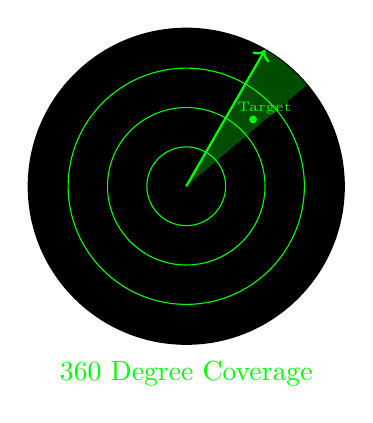
\begin{tikzpicture}
    % PPI Screen
    \draw[thick, fill=black] (0,0) circle (2);
    \draw[green, thin] (0,0) circle (0.5);
    \draw[green, thin] (0,0) circle (1);
    \draw[green, thin] (0,0) circle (1.5);
    
    % Sweep
    \draw[green, thick, ->] (0,0) -- (60:2);
    \fill[green, opacity=0.3] (0,0) -- (60:2) arc (60:40:2) -- cycle;
    
    % Targets
    \fill[green] (45:1.2) circle (0.05);
    \node[green, font=\tiny] at (45:1.4) {Target};
    
    \node[green, below] at (0,-2.1) {360 Degree Coverage};
\end{tikzpicture}
\end{answerdiagram}

\textbf{Features:}
\begin{itemize}
    \item Map-like display in polar coordinates (Range and Azimuth).
    \item Center of screen = Radar location.
    \item Sweep rotates in sync with antenna.
    \item Used in Air Traffic Control and Navigation.
\end{itemize}
\end{solutionbox}

\begin{mnemonicbox}
\mnemonic{PPI Provides Perfect Position Information}
\end{mnemonicbox}

\questionmarks{5(c)}{7}{Explain the basic pulse radar system with a block diagram.}

\begin{solutionbox}
\textbf{Pulse Radar System:}

\begin{answerdiagram}{Basic Pulse Radar}
\begin{tikzpicture}[auto, node distance=1.5cm]
    \node [gtu block] (sync) {Synchronizer\\(Timer)};
    \node [gtu block, right=of sync] (mod) {Modulator};
    \node [gtu block, right=of mod] (tx) {Transmitter};
    \node [gtu block, right=of tx] (dup) {Duplexer};
    \node [gtu input, right=of dup] (ant) {Antenna};
    
    \node [gtu block, below=of dup] (rx) {Receiver};
    \node [gtu block, left=of rx] (disp) {Display\\(Indicator)};
    
    \draw [gtu arrow] (sync) -- (mod);
    \draw [gtu arrow] (mod) -- (tx);
    \draw [gtu arrow] (tx) -- (dup);
    \draw [gtu arrow] (dup) -- (ant);
    \draw [gtu arrow] (ant) -- node[right] {Echo} (dup);
    \draw [gtu arrow] (dup) -- (rx);
    \draw [gtu arrow] (rx) -- (disp);
    \draw [gtu arrow] (sync) -| (disp);
    
    \node [right=0.5cm of ant] (target) {Target};
    \draw [gtu dashed arrow] (ant) -- (target);
    \draw [gtu dashed arrow] (target) to[bend left] (ant);
\end{tikzpicture}
\end{answerdiagram}

\textbf{Functions:}
\begin{itemize}
    \item \keyword{Synchronizer}: Controls timing of pulses.
    \item \keyword{Modulator}: Triggers transmitter.
    \item \keyword{Transmitter}: Generates high power RF pulses.
    \item \keyword{Duplexer}: Switches antenna between Tx and Rx (Protects receiver).
    \item \keyword{Receiver}: Amplifies weak echoes (Superheterodyne).
\end{itemize}

\textbf{Range Equation:} $R = cT/2$, where $T$ is round trip time.
\end{solutionbox}

\begin{mnemonicbox}
\mnemonic{Pulse Radar Properly Processes Reflected signals}
\end{mnemonicbox}

\orquestionmarks{5(a)}{3}{List the application of microwave frequency.}

\begin{solutionbox}
\textbf{Applications:}

\begin{answertable}{Microwave Uses}
\begin{tabulary}{\linewidth}{|L|L|}
\hline
\textbf{Field} & \textbf{Applications} \\ \hline
\keyword{Communication} & Satellite, Mobile, WiFi, Bluetooth \\ \hline
\keyword{RADAR} & Navigation, Weather forecasting, Defense \\ \hline
\keyword{Industrial} & Heating, Drying, Material testing \\ \hline
\keyword{Medical} & Diathermy, Cancer treatment (Hyperthermia) \\ \hline
\keyword{Domestic} & Microwave Ovens (2.45 GHz heating) \\ \hline
\keyword{Scientific} & Radio Astronomy, Particle Accelerators \\ \hline
\end{tabulary}
\end{answertable}
\end{solutionbox}

\begin{mnemonicbox}
\mnemonic{Microwaves Serve Many Applications Perfectly}
\end{mnemonicbox}

\orquestionmarks{5(b)}{4}{Compare PULSED RADAR and CW RADAR.}

\begin{solutionbox}
\textbf{Comparison:}

\begin{answertable}{Pulsed vs CW Radar}
\begin{tabulary}{\linewidth}{|L|L|L|}
\hline
\textbf{Parameter} & \textbf{Pulsed RADAR} & \textbf{CW RADAR} \\ \hline
\keyword{Signal} & Short pulses & Continuous Wave (Sine) \\ \hline
\keyword{Range} & Measures Range ($ct/2$) & Cannot measure Range (needs FM) \\ \hline
\keyword{Velocity} & Poor velocity measurement & Excellent (Doppler Effect) \\ \hline
\keyword{Power} & High Peak Power & Low Average Power \\ \hline
\keyword{Complexity} & Higher (Duplexer needed) & Simpler (Separate Antennas usually) \\ \hline
\keyword{Blindness} & Blind range (width dependent) & No blind range \\ \hline
\end{tabulary}
\end{answertable}
\end{solutionbox}

\begin{mnemonicbox}
\mnemonic{Pulsed measures Range, CW measures Velocity}
\end{mnemonicbox}

\orquestionmarks{5(c)}{7}{Explain MTI Radar with the block diagram.}

\begin{solutionbox}
\textbf{Moving Target Indication (MTI) Radar:}

\begin{answerdiagram}{MTI Block Diagram}
\begin{tikzpicture}[auto, node distance=1.5cm]
    \node [gtu block] (tx) {Tx};
    \node [gtu block, below=of tx] (rx) {Mixer};
    \node [gtu block, right=of tx] (dup) {Duplexer};
    \node [gtu input, right=of dup] (ant) {Ant};
    
    \node [gtu block, left=of tx] (pa) {Power Amp};
    \node [gtu block, left=of pa] (mod) {Modulator};
    
    \node [gtu block, below=of mod] (stalo) {STALO};
    \node [gtu block, below=of stalo] (coho) {COHO};
    
    \node [gtu block, below=of rx] (phasedet) {Phase\\Detector};
    \node [gtu block, right=of phasedet] (delay) {Delay Line};
    \node [gtu block, right=of delay] (sub) {Subtractor};
    \node [gtu output, right=of sub] (ind) {Indicator};
    
    \draw [gtu arrow] (stalo) -- (rx);
    \draw [gtu arrow] (stalo) -- (pa); % simplified connection
    \draw [gtu arrow] (dup) -- (rx);
    \draw [gtu arrow] (rx) -- (phasedet);
    \draw [gtu arrow] (coho) -- (phasedet);
    
    \draw [gtu arrow] (phasedet) -- (delay);
    \draw [gtu arrow] (phasedet) -- (sub); % direct path
    \draw [gtu arrow] (delay) -- (sub);    % delayed path
    \draw [gtu arrow] (sub) -- (ind);
\end{tikzpicture}
\end{answerdiagram}

\textbf{Principle (Doppler Effect):}
\begin{itemize}
    \item \keyword{Stationary Targets}: Returns have constant phase pulse-to-pulse.
    \item \keyword{Moving Targets}: Returns have changing phase due to Doppler shift.
\end{itemize}

\textbf{Operation:}
\begin{itemize}
    \item \keyword{Delay Line Canceler}: Compares current echo with previous echo (delayed by one PRT).
    \item Subtractor output: $V(t) - V(t-T)$.
    \item Stationary targets cancel out ($V_{now} = V_{prev}$). Moving targets remains.
\end{itemize}

\textbf{Blind Speed}: Speeds where phase shift is $360^\circ$ multiples result in cancellation (Blindness).
\end{solutionbox}

\begin{mnemonicbox}
\mnemonic{MTI Makes Targets Identifiable by Movement}
\end{mnemonicbox}

\end{document}
